\section{Experimental Evaluation}

We evaluate all the models developed in NetLearner on the 5-class NSL-KDD task and the 2-class UNSW-NB15 task using the following metrics.
\begin{itemize}
    \item \textbf{Accuracy} is the percentage of correctly classified connections
        over the total number of connections in the dataset:
        \begin{align}
            A = \frac{\text{True Positives + True Negatives}}{\text{Number of Instances}}
        \end{align} 
        Accuracy is not suitable for evaluating imbalance datasets where the number
        of records of one class is extremely larger than the number of
        records of another class.
        In the NSL-KDD dataset, the number of available U2R records (i.e., 67)
        is two orders of magnitude less than the number of records in other classes
        (i.e., 9711, 7458, 2887 and 2121).
        Therefore, we also consider the precision and recall.
    \item \textbf{Precision} is the percentage of the correctly classified positives over
        the total number of positives predicted by the classifier.
                \begin{align}
                    P = \frac{\text{True Positives}}{\text{True Positives} + \text{False Positives}}
                \end{align}
    \item \textbf{Recall} is the percentage of the correctly classified positives over
        the total number of relevant elements.
                \begin{align}
                    R = \frac{\text{True Positives}}{\text{True Positives} + \text{False Negatives}}
                \end{align}
\end{itemize}
%The weight for each class is determined by its proportion in the test dataset,
%namely [0.431, 0.107, 0.339, 0.018, 0.105] for class [Normal, Probe, DoS, U2R, R2L] respectively.
%Besides, we also calculate the confusion matrices of the classification results when applying
%different approaches on both task's test datasets.
%In a confusion matrix table, the $i$th row represents the instances of class $i$,
%while the $j$th column represents the instances predicted by the classifier as class $j$.
%It is called confusion matrix because it is useful for visualizing how a classifier
%is confusing one class with other classes.
%Due to page space limit, here we only present the most straightforward
%and relatively more important metric accuracy.
%Statistics regarding precision, recall and confusion matrices can be found
%in our detailed technical report~\cite{OurWonReport} and our codebase~\cite{NetLearner}.

We train an radial basis function kernel support vector machine (SVM) % using the approach in ~\cite{ScikitLearnSVM},
and report its accuracy with the multilayer perceptron (MLP) model,
the restricted Boltzmann machine fine-tuned neural network (RBM),
the sparse autoencoder fine-tuned neural network (SAE),
and the wide linear classifier and deep neural network combined model (WnD).

It is critical to search the optimal hyper-parameters that fit the problem domain and model before training machine learning models. We first manually set all the hyper-parameters, including the number of layers, number of neurons in each layer, learning rate, and batch size, to be identical across all the models.
We then use 5-fold cross-validation on the training datasets to determine the optimal training time $T$
for each model.
Finally, we train the model for $T$ epochs and report the metrics on the testing dataset,
which is not touched during the training phase.
Determining the training time (model complexity) by cross-validation with fixed common hyper-parameters
ensures that the deep learning models are neither overfitting nor underfitting.
We plot the 5-fold cross validation loss of MLP in Figure~\ref{CDL:Fig:LossHistory}.
We can see that the validation loss converges to approximately 0.02 after 140 epochs, even though the training loss still decreases,
and the optimal training time that validation loss is minimized is at $T \approx 150$.
In this case, we train the MLP on NSL-KDD train dataset for exactly 150 epochs and report its metrics on NSL-KDD test dataset.

The accuracies of all considered classifier are shown in Figure~\ref{CDL:Fig:CompAccuracyNSL} for the NSL-KDD task and
Figure~\ref{CDL:Fig:CompAccuracyUNSW} for the UNSW-NB15 task.
In the 2-class UNSW-NB15 dataset,
the volumes of normal and attacking traffic are nearly balanced (i.e., 37,000 normal v.s. 45,332 attacking records).
Therefore, we only report the precision and recall for the attacking traffics in Figure~\ref{CDL:Fig:CompAccuracyUNSW}.
For the 5-class NSL-KDD task, we adopt the approach in~\cite{STL-NIDS}
to calculate the weighted precisions and recalls, and plot them together with accuracy in Figure~\ref{CDL:Fig:CompAccuracyNSL}.
The per-class precisions and recalls are also listed in Table~\ref{CDL:Tab:PrecisionRecall}.

For the NSL-KDD task, all classifiers achieve high training accuracy (no less than 99\%).
However, all classifiers show a gap between training accuracy and testing accuracy (as low as 78.4\%).
As the representative of the classic machine learning approach, SVM achieves a 78.5\% accuracy
comparable to the deep learning models.
Note that our SAE model achieves the same accuracy performance to~\cite{STL-NIDS}, which is the best among all the considered models (79.2\%).
RBM, SAE, and WnD all outperform MLP for two different reasons.
RBM and SAE provide their underlying MLP with better initial weights in the first layer
than randomly generated numbers.
WnD has a slightly higher accuracy because of the extra linear model.
Table~\ref{CDL:Tab:PrecisionRecall} shows two remarkable facts.
SVM performs better at Probe attacks (93\% precision and 82\% recall)
than all the neural networks ($\approx$ 85\% precision and $\leq$ 70\% recall),
However, it suffers hugely on U2R attacks ($\approx$ 6\% precision and recall).
On the other hand, the neural networks (MLP, RBM, SAE and WnD) miss many U2R attacks ($\leq$ 6\% recall),
but they have much higher reliability in identifying these attacking traffic ($\approx$ 60\% precision).

For the UNSW-NB15 task, the average accuracies of RBM, SAE and WnD are
all higher than MLP for the same reason mentioned in the NSL-KDD task.
We notice WnD has significantly improved MLP's performance by around 5\%.
Different from the NSL-KDD task, the training accuracies of all the approaches are mediocre
(up to 94.4\%) in contrast to the NSL-KDD case where the training accuracy of every model is more than 99\%.
The harder UNSW-NB15 training dataset is one primary reason that the testing accuracies of the UNSW-NB15 task
are higher than that of the NSL-KDD task, since classifiers only have access to the training dataset.
Therefore, even though SVM has an equivalent training accuracy to the neural networks (93\% v.s. 94\%),
its testing accuracy falls far behind by 5\% (comparing to MLP) to 9\% (comparing to WnD),
showing the superior generalization capability of the deep neural network models.
The detection alarms are mostly correct for every classifier,
due to the high recall values $\geq$ 97\%, and the deep learning models have better precision ($\geq$ 81\%) than SVM (75\%).

\begin{figure}[h]
    \centering
    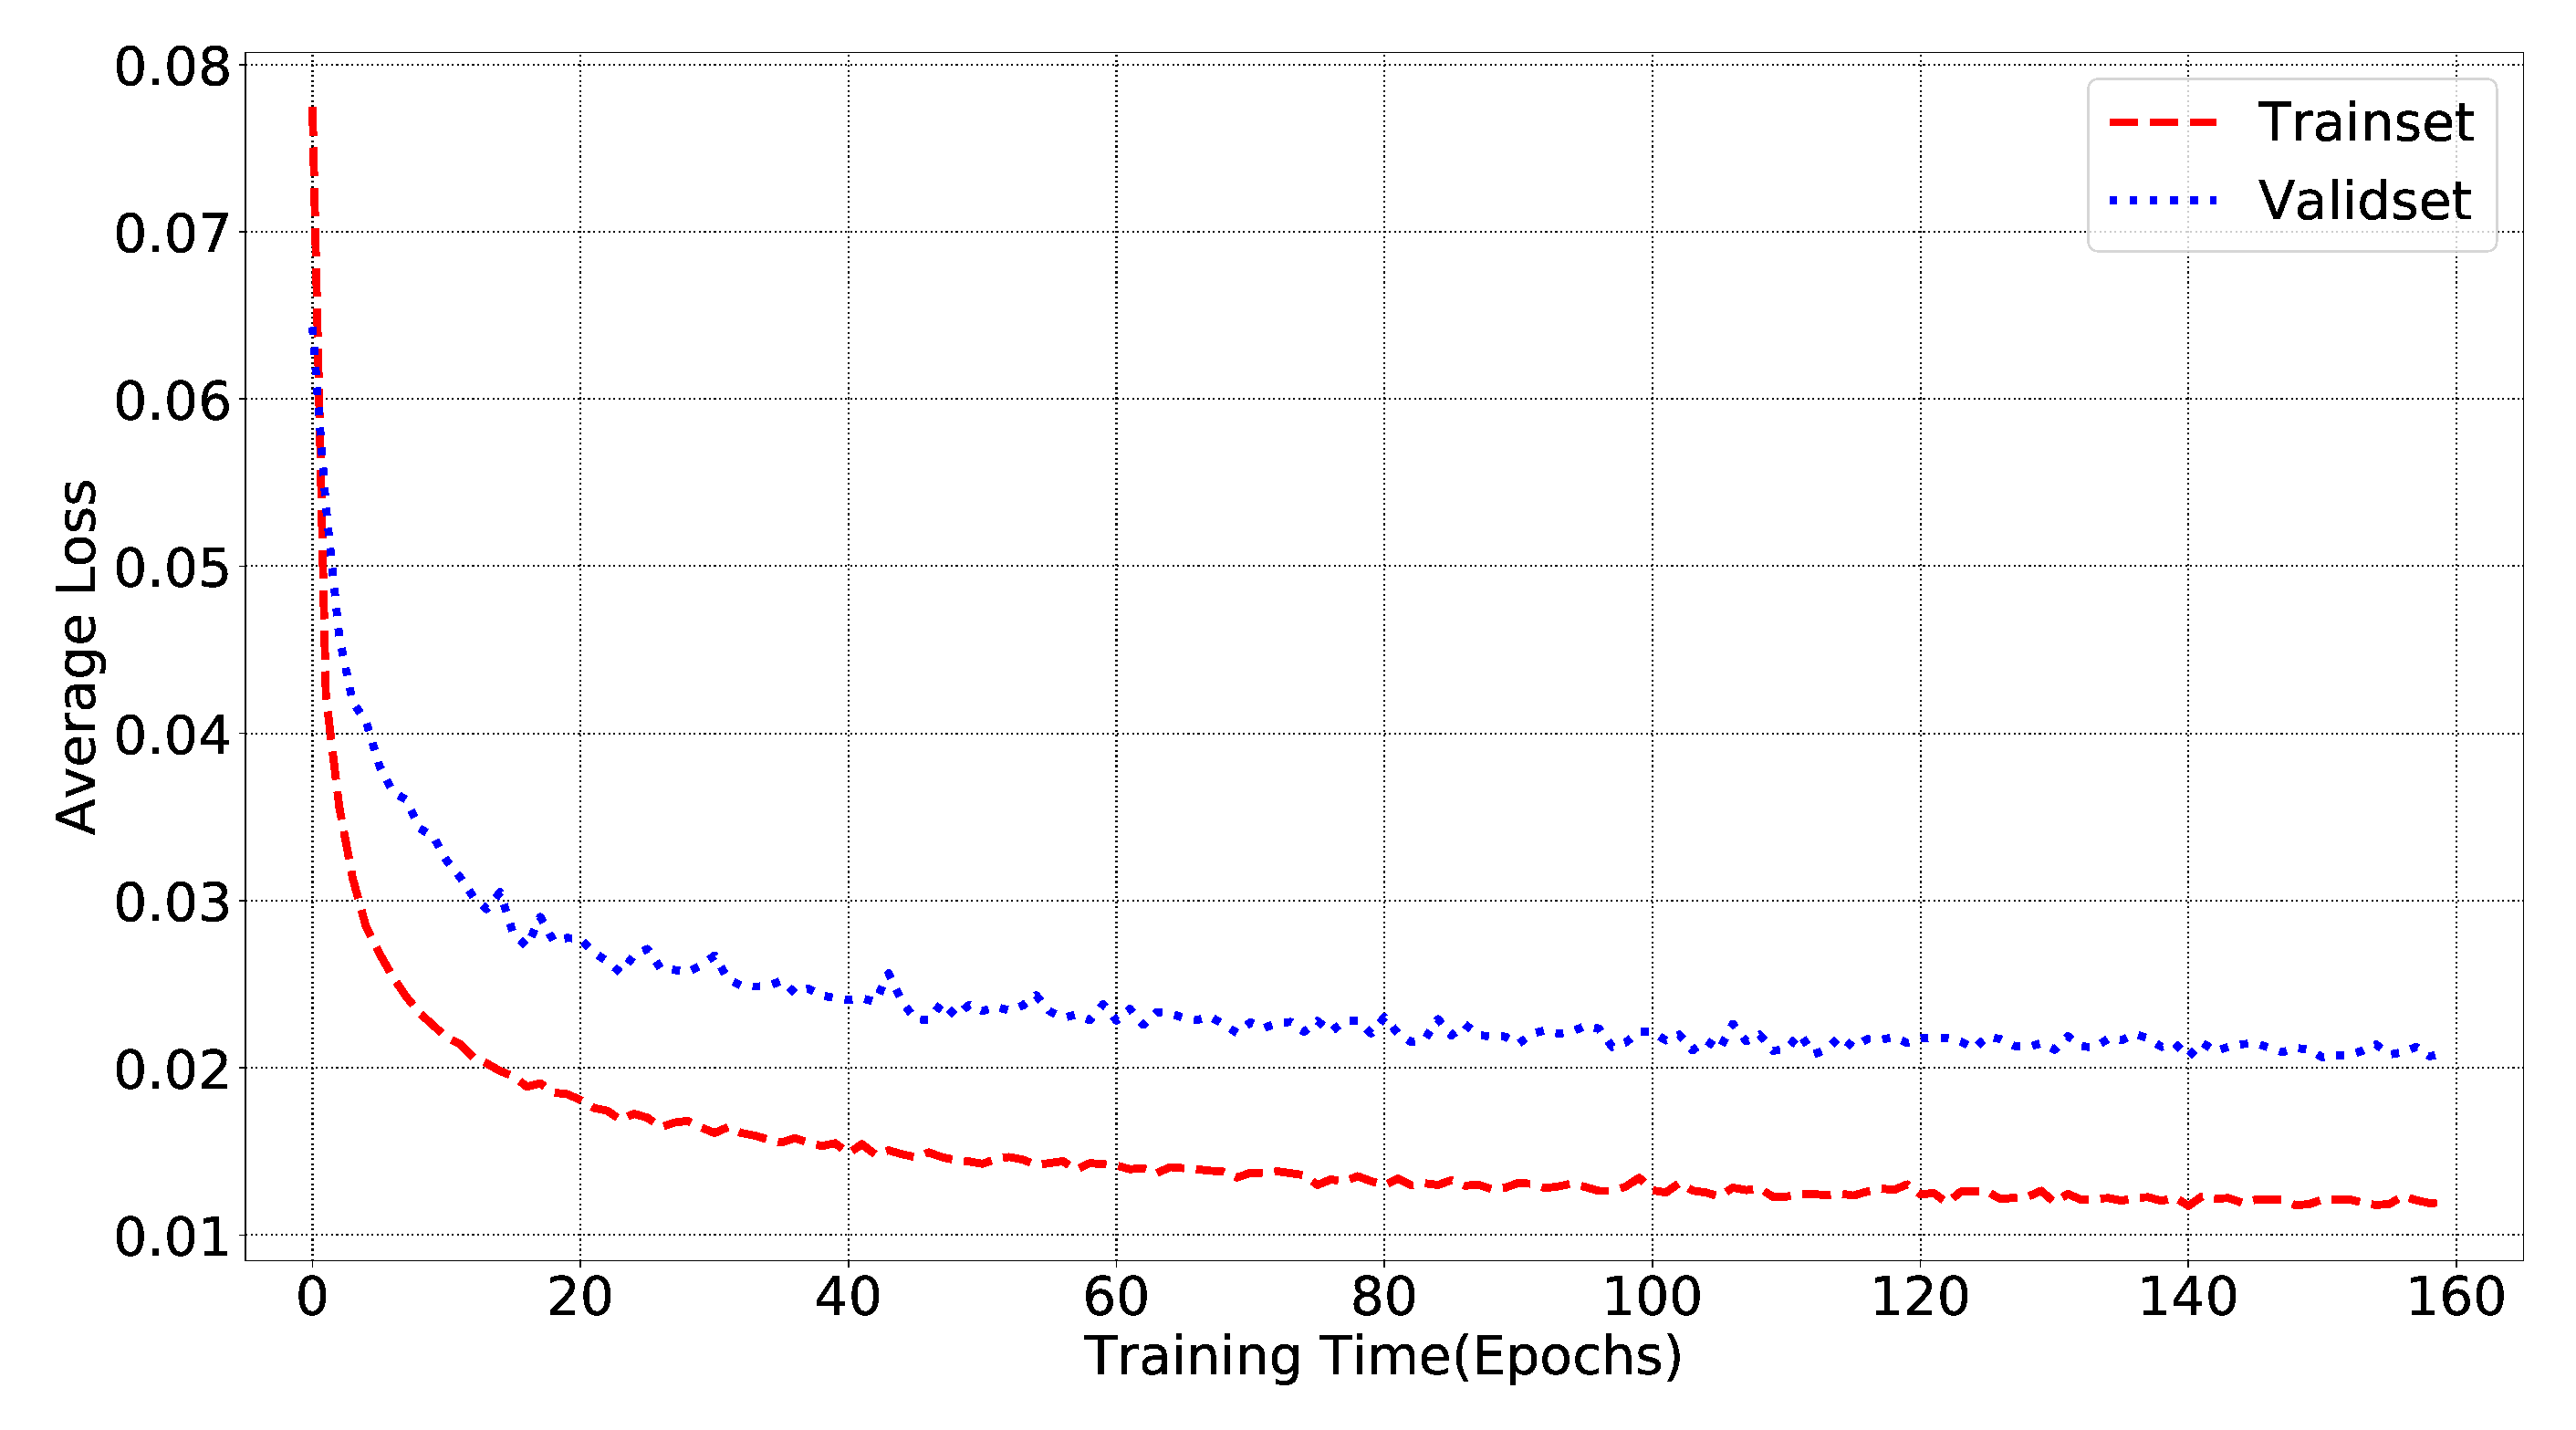
\includegraphics[width=0.9\textwidth]{CompareDL/figures/history.eps}
    \caption{History of MLP's Average Loss During Cross Validation}
    \label{CDL:Fig:LossHistory}
\end{figure}

\begin{figure}[h]
    \centering
    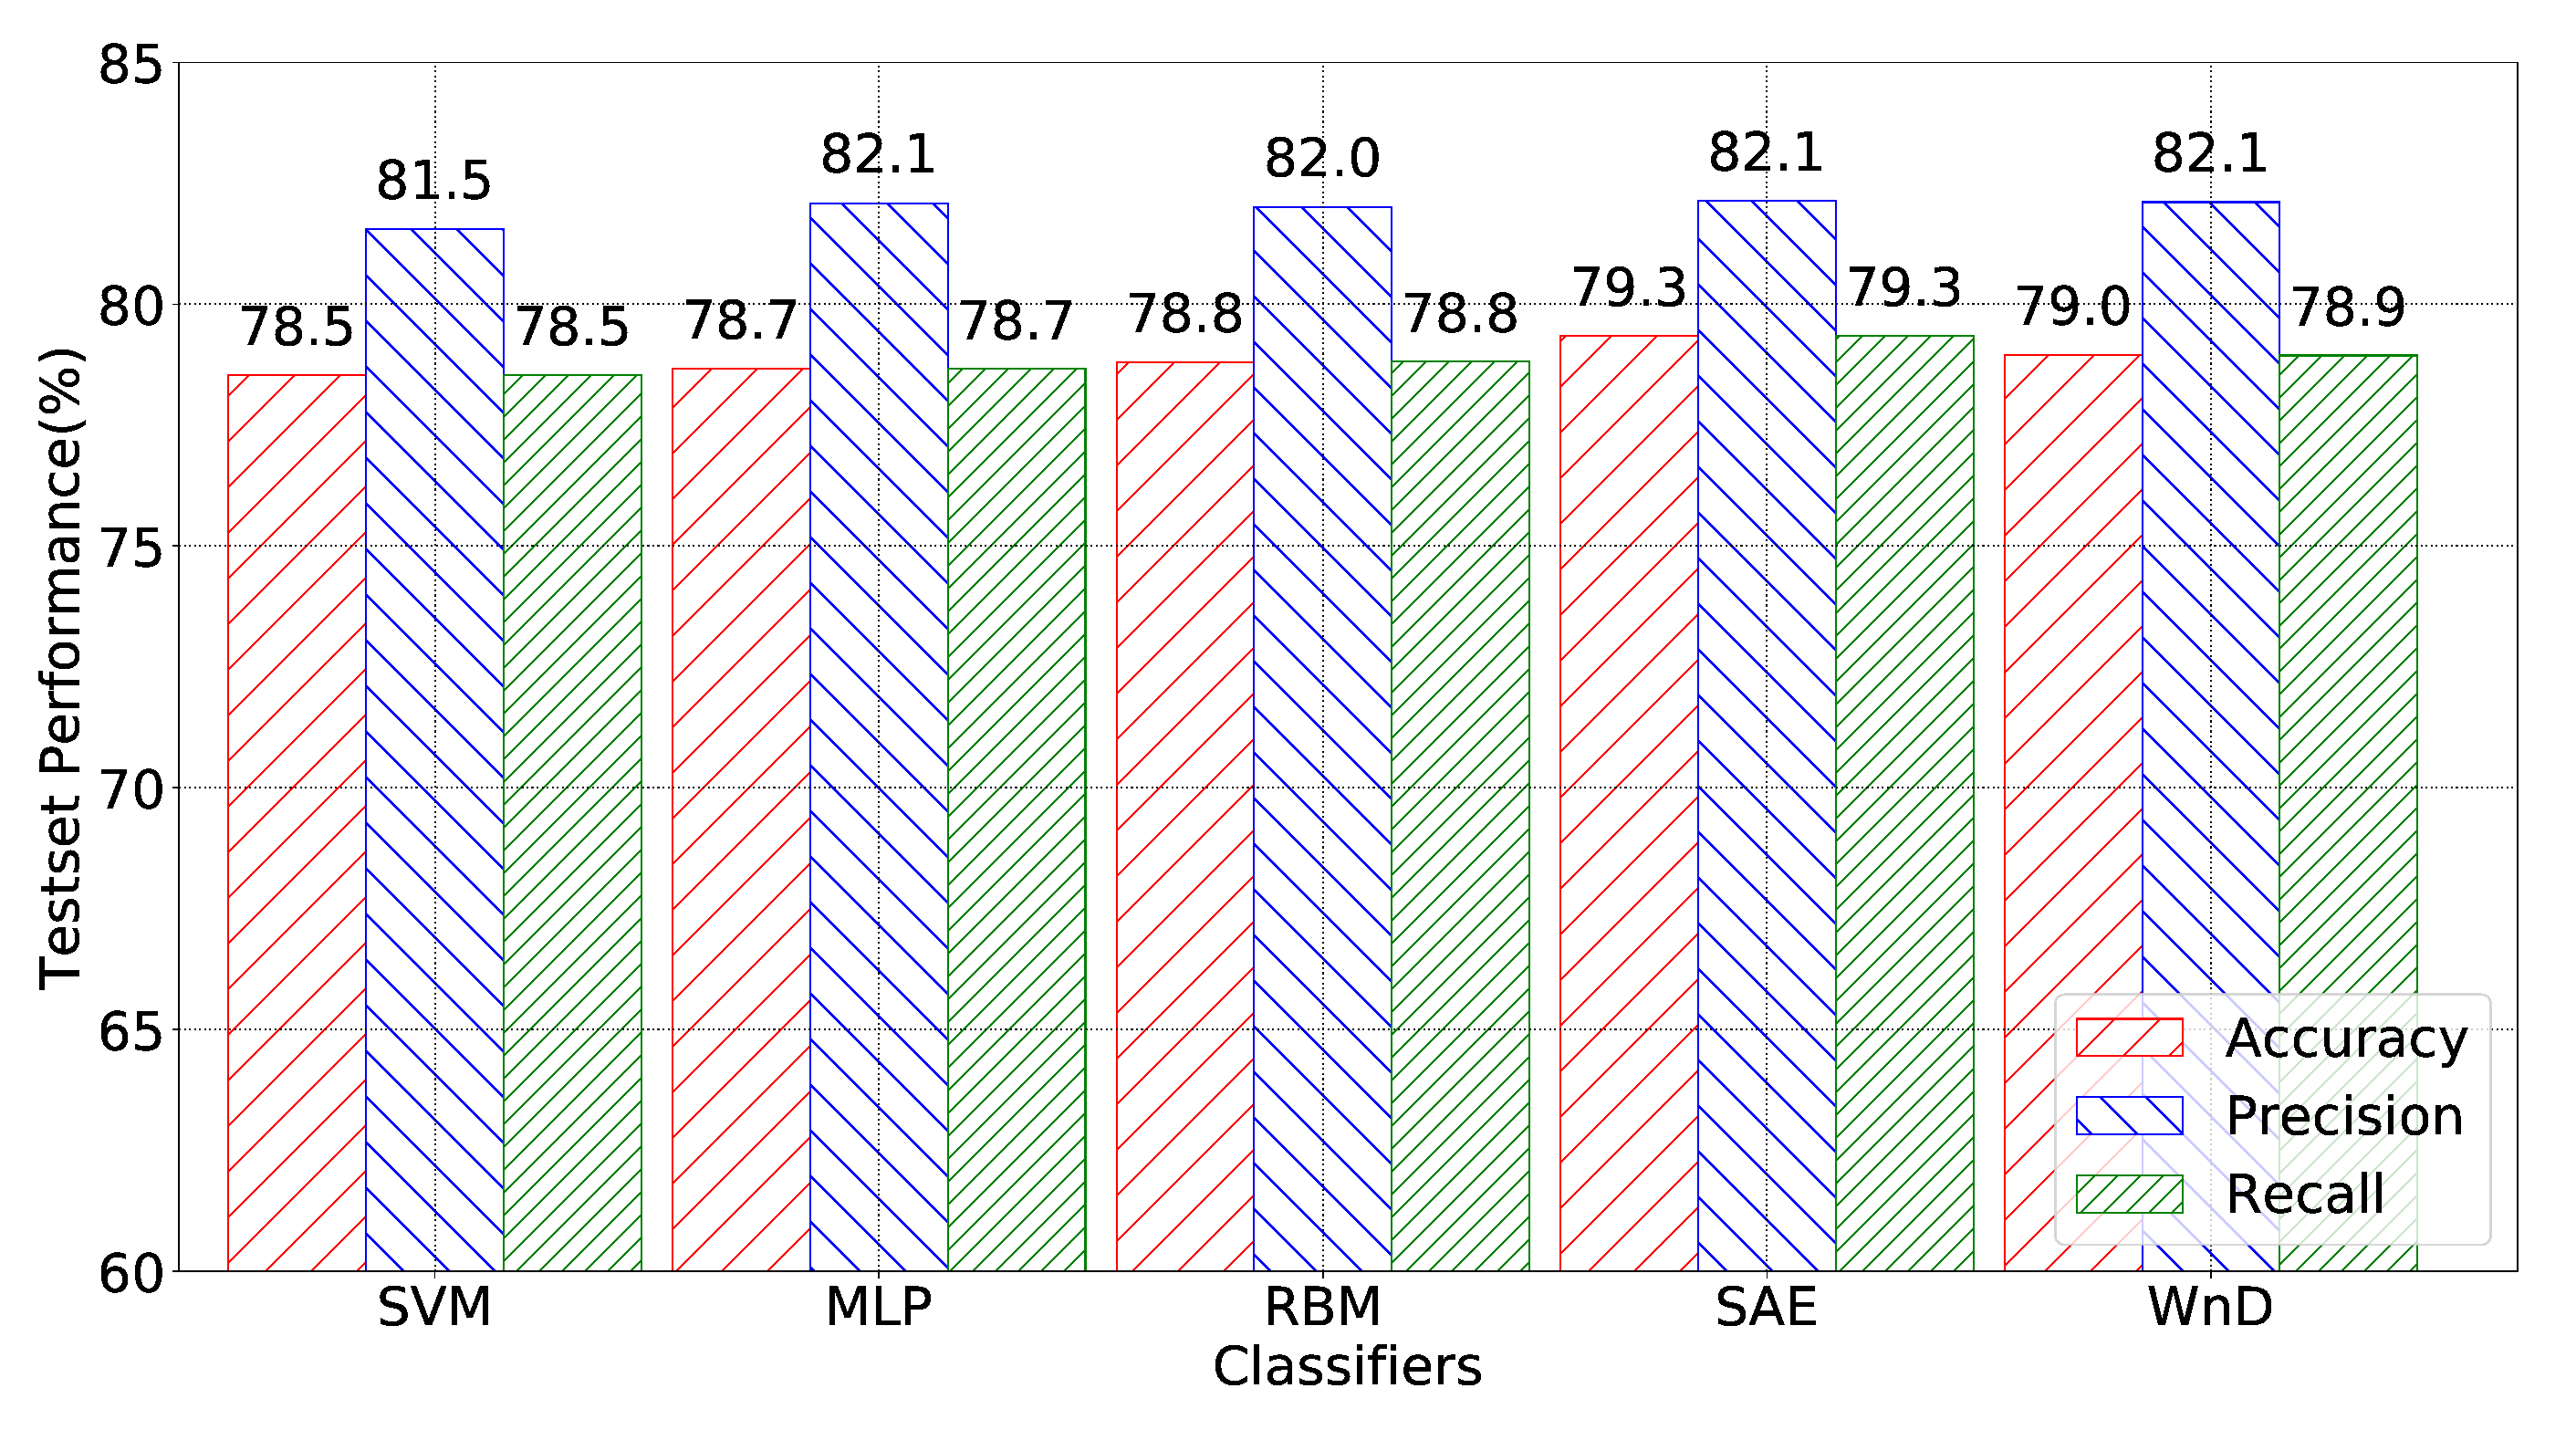
\includegraphics[width=0.9\textwidth]{CompareDL/figures/comp_accuracy_nsl.eps}
    \caption{Metrics Comparison, NSL-KDD Task}
    \label{CDL:Fig:CompAccuracyNSL}
\end{figure}

\begin{figure}[h]
    \centering
    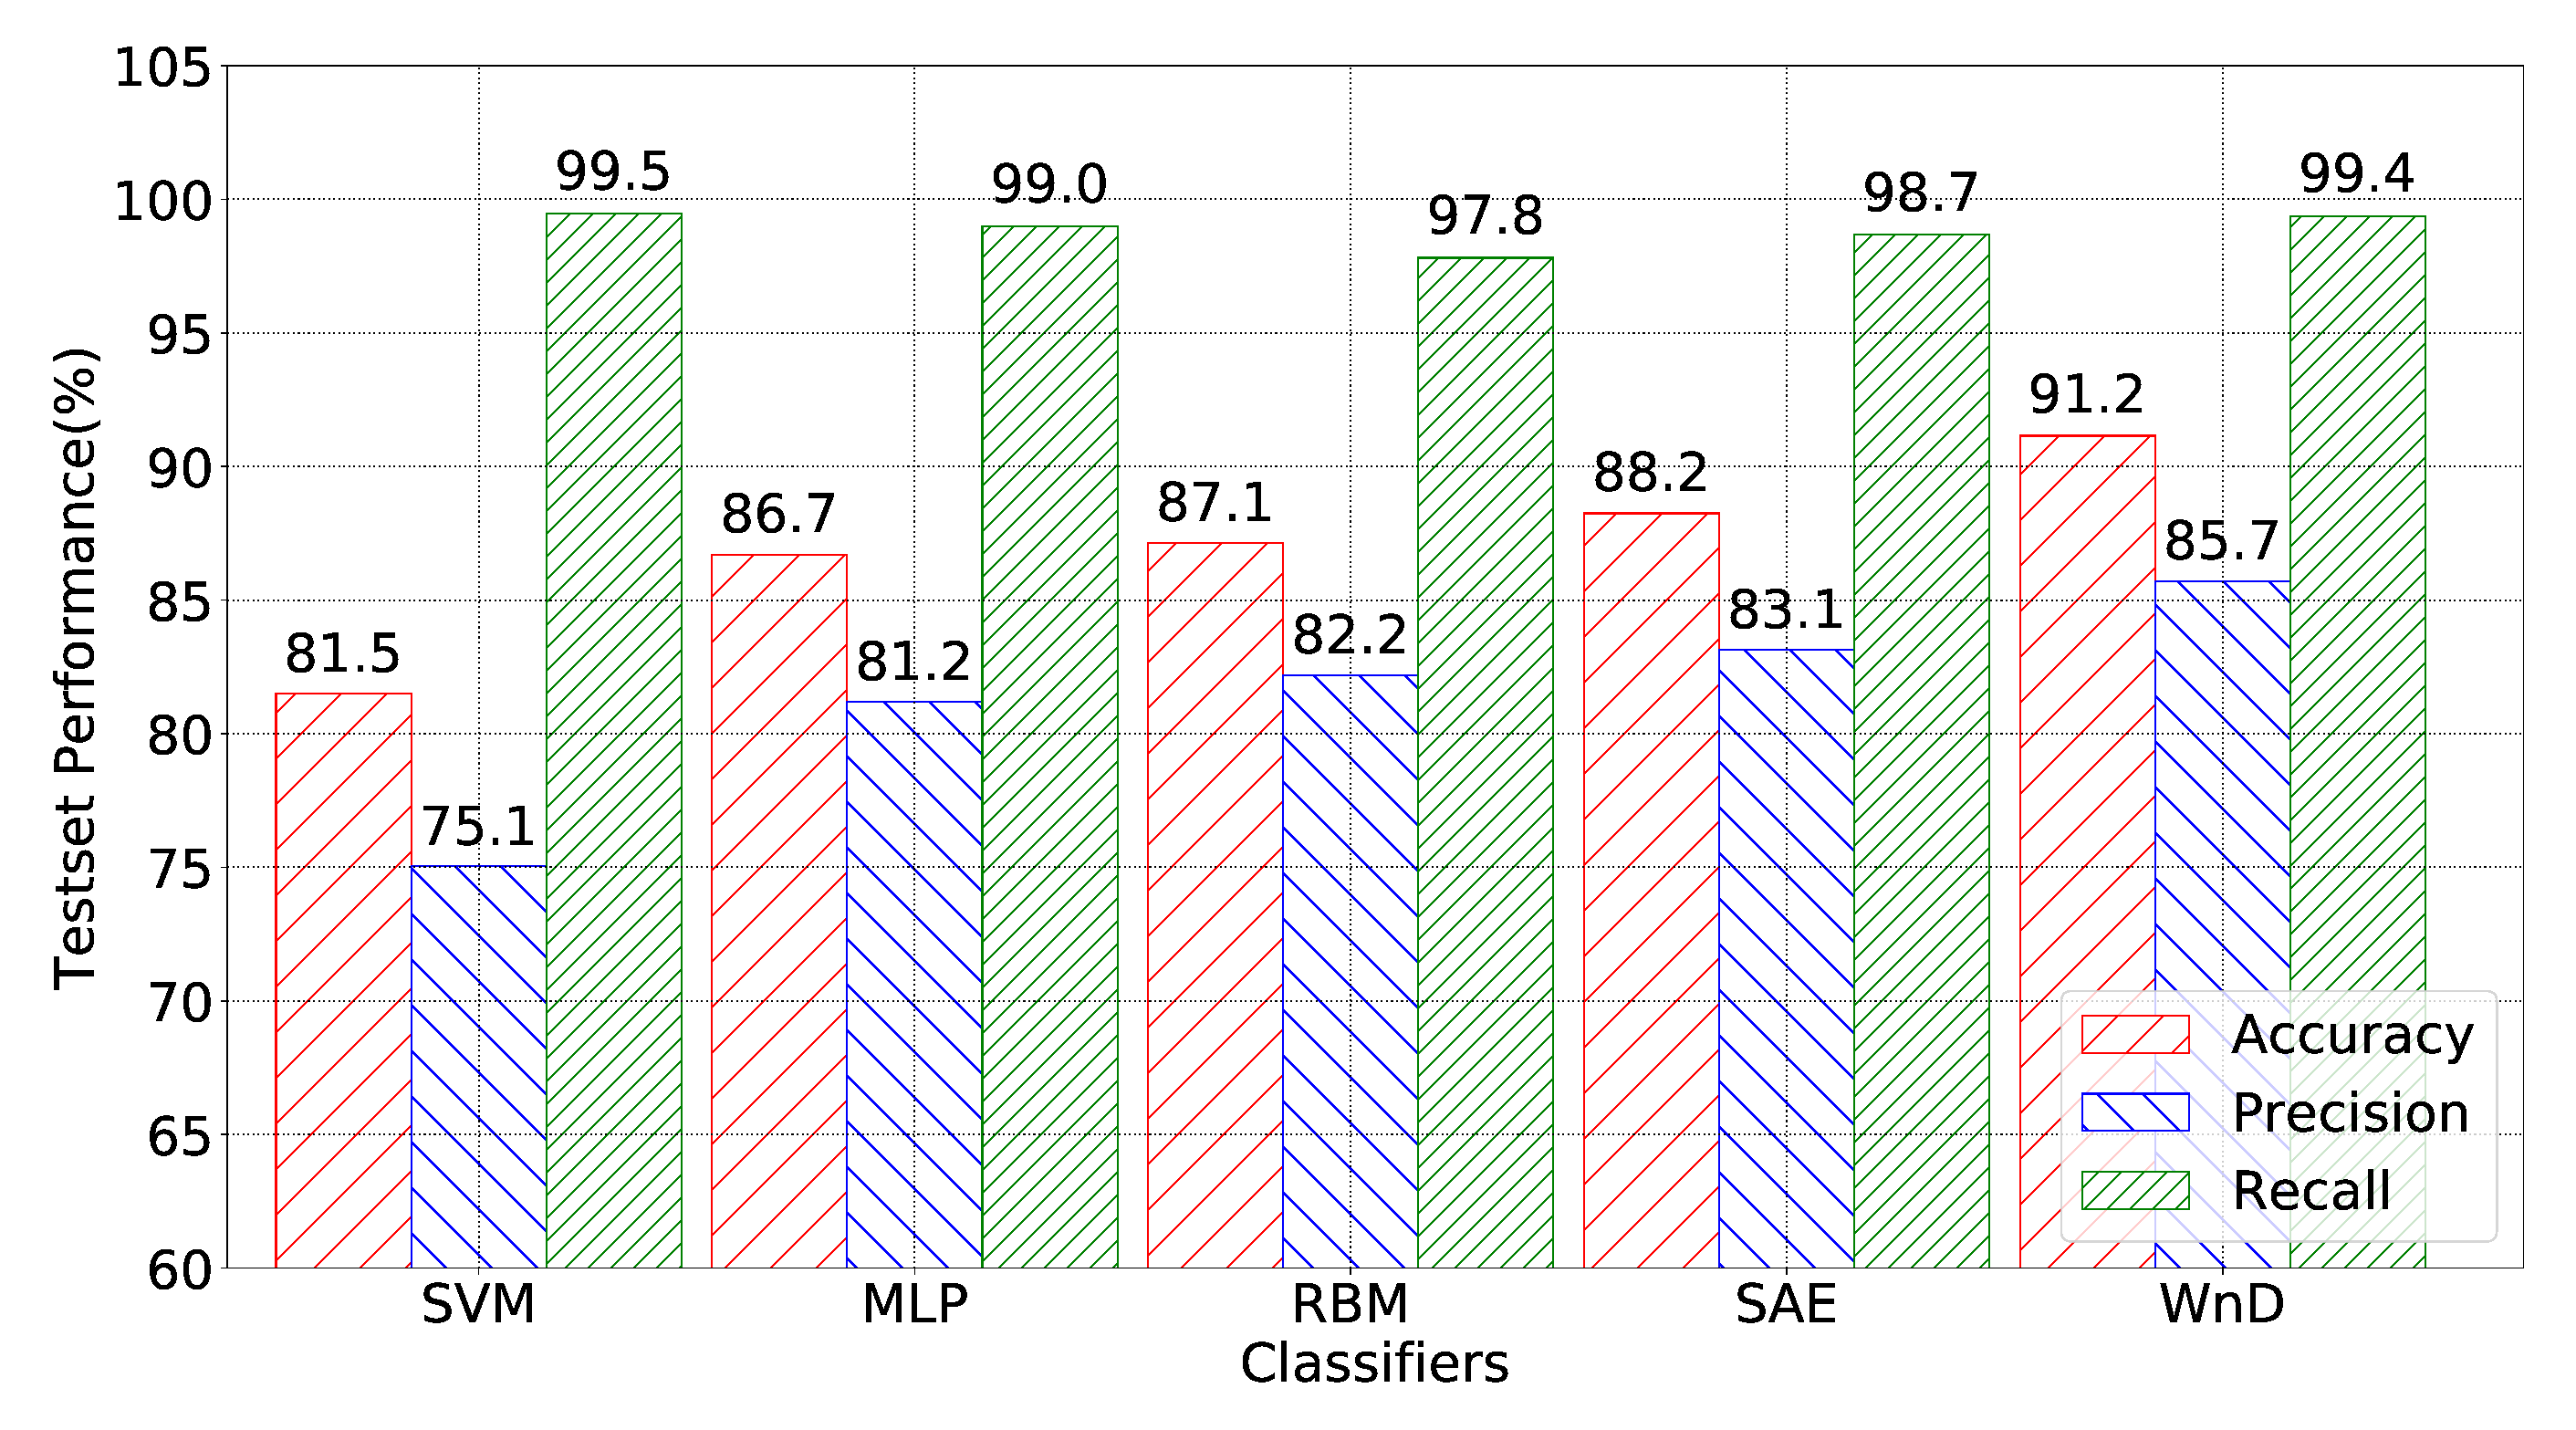
\includegraphics[width=0.9\textwidth]{CompareDL/figures/comp_accuracy_unsw.eps}
    \caption{Metrics Comparison, UNSW-NB15 Task}
    \label{CDL:Fig:CompAccuracyUNSW}
\end{figure}

\begin{table}[tbp]
    \centering
    \caption{Per-class Precision/Recall on the NSL-KDD Task}
    \label{CDL:Tab:PrecisionRecall}
    \begin{tabular}{c|c|ccccc}
        \hline
        \hline
                             &            & \multicolumn{5}{c}{Traffic Class} \\
        \cline{3-7}
                             &            & Normal & DoS   & Probe & U2R   & R2L \\
        \hline
        \multirow{2}{*}{SVM} & Precision  & 72.82  & 75.27 & 93.85 &  6.32 & 96.65 \\
        \cline{2-2}
                             & Recall     & 96.18  & 72.16 & 82.16 &  6.06 & 13.34 \\
        \hline
        \multirow{2}{*}{MLP} & Precision  & 69.18  & 95.49 & 85.58 & 59.52 & 92.01 \\
        \cline{2-2}
                             & Recall     & 96.66  & 82.31 & 69.28 &  6.31 & 15.03 \\
        \hline
        \multirow{2}{*}{RBM} & Precision  & 69.41  & 95.41 & 85.23 & 41.51 & 93.86 \\
        \cline{2-2}
                             & Recall     & 96.81  & 83.89 & 64.74 &  5.56 & 15.48 \\
        \hline
        \multirow{2}{*}{SAE} & Precision  & 70.20  & 95.63 & 84.70 & 65.00 & 87.76 \\
        \cline{2-2}
                             & Recall     & 96.92  & 83.34 & 70.56 &  3.28 & 16.29 \\
        \hline
        \multirow{2}{*}{WnD} & Precision  & 70.08  & 95.59 & 84.02 & 60.34 & 91.57 \\
        \cline{2-2}
                             & Recall     & 96.88  & 83.64 & 67.84 &  4.53 & 15.34 \\
        \hline
    \end{tabular}
\end{table}

